%UNIT 1: QUALITATIVE AND GRAPHICAL APPROACHES
% Is first part of original 01.tex
%%%%%%%%%%%%%%%%%%%%%%%%%%%
%%%% Put the following at the top of each .tex file  %
\pagestyle{fancy}
\renewcommand{\theUnit}{3}
\ifthenelse{\isundefined{\UnitPageNumbers}}{}{\setcounter{page}{1}}
\rhead{Carlton and Devore Chapter \theUnit: Continuous Random Variables}
\lhead{Math 3382: Statistical Theory}
%\lhead{
\includegraphics[width=1.25cm]{CUDenver-Logo.png}}
\rfoot{\mypage}
\cfoot{
\includegraphics[width=2.25cm]{CUDenver-Logo-coverpage.png}}
\lfoot{Adam Spiegler}
\fancypagestyle{firstfooter}{\footskip = 50pt}
\renewcommand{\footrulewidth}{.4pt}
%%%%%%%%%%%%%%%%%%%%%%%%%%%
\vspace*{-20pt} \thispagestyle{firstfooter}

\pagebegin{Introduction to Continuous Random Variables}

A manufacturer of lithium batteries measures the weight of each box they ship out to customers. Let $X$ denote the weight (in pounds) of a randomly selected shipment. It is possible that $X=8$ or $X=9$, but the weight could potentially be any value (greater than 0) such as $8.3671$ pounds if they want to be really precise. Recall the previous definition of a random variable below.

\begin{tcolorbox}
\begin{definition}\label{def:crv}
A \textbf{\colorb{random variable}} is a mapping
\[ X: \Omega \to \mathbb{R} \]
that assigns a real number $X(\omega)$ to each outcome $\omega \in \Omega$.
\end{definition}

\bi
\ii With a discrete random variable, the sample space is mapped to the integers (or a subset of the integers).
\ii With a continuous random variable, the sample space is mapped to an interval of values in $\mathbb{R}$.
\ei

\end{tcolorbox}

\bb
\begin{multicols}{2}

\ii Imagine the GPA distribution for all students at a university follows a \textbf{\colorb{uniform distribution}} with GPA's 
of 0 and 4 being the smallest and largest GPA's possible. \label{gpa-uniform}

\bb
\ii Write a formula for probability density function $f_X(x)$ for the uniform distribution. \vspace{0.5in}
\ii What proportion of students earned a GPA between $3$ and $3.5$?
\ee

\columnbreak

\begin{center}
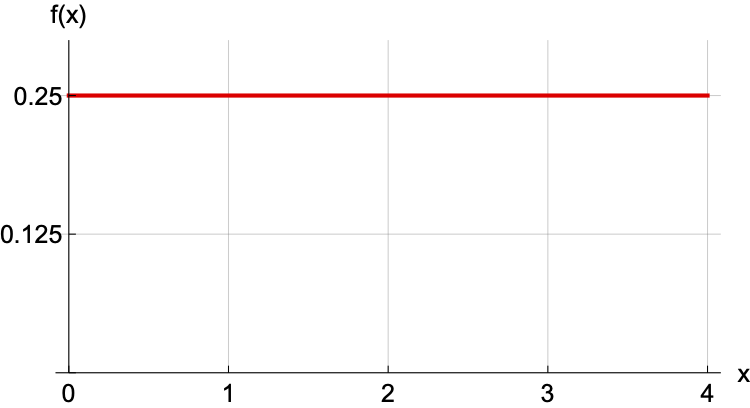
\includegraphics[width=0.45\tw]{06/06gpa-unif.pdf}
\end{center}

\end{multicols} \vspace{0.5in}

\begin{multicols}{2}
\ii The graph of $f_X(x)$ below shows the probability density function for the GPA's of all students at a university.\label{gpa-v}

\bb
\ii What proportion of students at the university have a GPA between 3 and 4? \vspace{0.5in}
\ii What proportion of students at the university have a GPA between 1 and 3?
\ee

\columnbreak

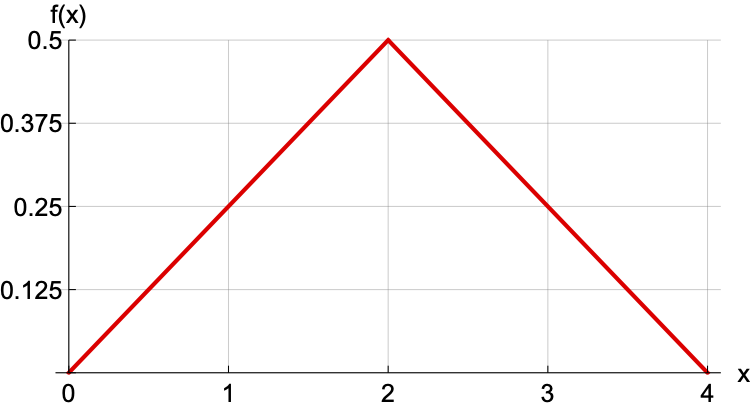
\includegraphics[width=0.5\tw]{06/06gpa-v.pdf}

\end{multicols} \vspace{0.5in}

\ee

\clearpage

\pagebegin{Probability Distributions}

\begin{tcolorbox}
\begin{multicols}{2}

\begin{definition}\label{def:pdf}
If $X$ is a \textbf{continuous} random variable, the \textbf{\colorb{probability density function (pdf)}}, denoted $f(x)$ satisfies the following properties:
\bi
\ii $f(x) \geq 0$ for all $x$,
\ii $\dsty \int_{-\infty}^{\infty} f(x) = 1$, and 
\ii $\dsty P(a < x < b) = \int_a^b f(x) \, dx$
\ei
\end{definition}

\columnbreak

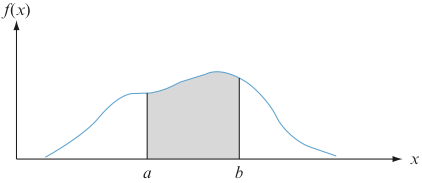
\includegraphics[width=0.5\tw]{06/06area1.png}
\end{multicols}
\end{tcolorbox}

\bb
\ii The probability of a transistor failing between time $x=a$ and $x=b$ months is given by the probability density function\label{transistor}
\[ f(x) = c \int_a^b e^{-cx} \, dx.\]
\bb
\ii If the probability of failure within the first six months, $0 < x < 6$, is 10\%, set up (but do not solve) an equation to find the value of $c$? \vfill
\ii Set up (but do not evaluate) an integral to represent the probability the transistor fails within the second six months ($6<x<12$)? \vfill
\ii Interpret the meaning of $P(X \leq 9)$ and $P(X < 9)$.\vfill
\ee
 \ee

\clearpage

\begin{tcolorbox}
\begin{definition}\label{def:cdf2}
If $X$ is a \textbf{continuous} random variable, the \textbf{\colorb{cumulative distribution function (cdf)}}, denoted $F(x)$ is
\[ P(X < x) = F(x) = \int_{-\infty}^x f(t) \, dt.\]
\textbf{\colorb{In other words, $F(x)$ is an antiderivative of $f$,} and \colorr{$f(x)$ is the derivative of $F(x)$}.}
\end{definition}
\end{tcolorbox}

\bb[resume]
\begin{multicols}{2}
\ii Match the graphs of the density functions (a), (b), and (c)  with the graphs of the cumulative distribution functions I, II, and III.\label{graph-match}
\columnbreak
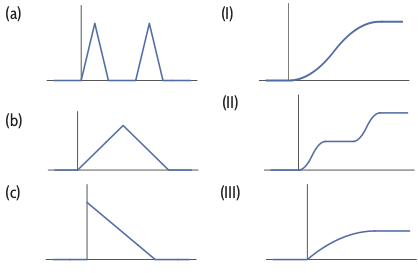
\includegraphics[width=0.5\tw]{06/06match.png}
\end{multicols}
\ee

%\clearpage

%\pagebegin{Cumulative Distribution Functions: Section 3.1}

%\bb[resume]
%\ii Decide if the function graphed in is a
%probability density function (pdf) or a cumulative distribution
%function (cdf).  Give reasons.  Find the value of $c$.  Sketch and
%label the other function.  (That is, sketch and label the cdf if the
%problem shows a pdf, and the pdf if the problem shows a cdf.)

%\begin{tasks}[counter-format = {(tsk[a])},label-offset = {0.8em},label-format = {\color{black}\bfseries}](2)
%\task 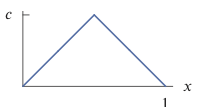
\includegraphics[width=0.4\tw]{06/06graph1.png}
%\task 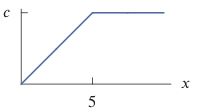
\includegraphics[width=0.4\tw]{06/06graph2.png}
%\end{tasks}
%\ee

\pagebegin{Mean, Variance, and Median}

\begin{tcolorbox}
\bi
\ii The \colorb{mean} of a continuous random variable is\label{def:mean}
\[ E(X) = \mu = \int_{-\infty}^{\infty} x \cdot f(x) \, dx.\]
\ii The \colorb{variance} of a continuous random variable is\label{def:variance}
\[ \Var(X) = E(X-\mu)^2 = E(X^2) - \big( E(X) \big)^2  \ \ \ \mbox{(this can be proven similar as with discrete case)}.\] 
\ii The \colorb{median} is the value $x$ such that $P(X < x) = 0.5$. Thus to find the median we solve the following for $x$:\label{def:median}
\[ F(x) = \int_{-\infty}^x f(t) \, dt = 0.5.\]
\ei
\end{tcolorbox}

\clearpage

\pagebegin{Practice}

\bb[resume]
\ii Consider the random variable with pdf
\[ f(x) = \left\{ \begin{array}{ll} \frac{x}{8}, & \hspace{0.2in} 0 \leq x \leq 4 \\ 0, &  \hspace{0.2in} \mbox{otherwise} \end{array} \right. .\]
\bb
\ii Sketch a graph of the pdf, $f$. \vfill
\ii Give a formula for the cdf, $F$, and sketch its graph. \vspace{1in}
\ii Calculate $P(X < 1)$ and illustrate this value on both of your graphs. \vspace{1in}
\ii Calculate $E(X)$. \vspace{1in}
\ii Give the median value and illustrate this value on both of your graphs. \vfill
\ee
\ee

